\chapter{Basic Topology}
  \label{chapter:Basic Topology}
    \section{Quick recap on Sets, Maps, and Equivalence classes}
      \subsection*{Set theory}
        A set is a well-defined collection of objects. The cardinality of a
        set $A$, denoted as $|A$, is the number of elements in the set. The
        elements in a set are unique, and the ordering of elements in a set
        doesn't matter. The set with no elements at all is known as the null
        set, denoted as $\phi$ or $\{\}$. Given a set $A$, we also have $A^c$
        as another set that contains all other elements that are not in $A$.
        $A^c$ is known as "$A$ complement".

        Given two sets $A$ and $B$, we can produce new sets from $A$ and $B$
        using the following operations \[\cap \quad \cup \quad \backslash \]
        known as the intersection, the union and the complement respectively.
        \begin{enumerate}
          \item{$A\cap B$: is a new set that contains elements that are in
          both $A$ and $B$.}
          \item{$A\cup B$: is a new set that contains elements that are in
          either $A$ or $B$.}
          \item{$A \backslash B$: is a new set that contains elements that
          are in $A$ but not in $B$. The complement is also sometimes written
          as $A - B$.}
        \end{enumerate}
        These operations obey De Morgan's laws. The two more important ones
        are: $(A \cup B)^c = A^c \cap B^c$ and $(A \cap B)^c = A^c \cup B^c$.
        There is also a very important theorem known as the
        "inclusion-exclusion" principle, which is only stated in name here
        but can be found in any introductory mathematics books.

        Suppose we have two sets $A$ and $B$. If $\forall b \in B,\, b \in
        A$, we say that $B \subset A$, or that $B$ is a subset of $A$. For a
        set $A$, the set of all its subsets is known as the power set of $A$,
        denoted as $\mathcal{P}(A)$. E.g, if $A = \{1,2,3\}$, then
        $\mathcal{P}(A) =$ $\{ \{\}, \{1\}, \{2\}, \{3\}, \{1,2\},
        \{2,3\},\{1,3\},\{1,2,3\}\}$. We can easily prove that
        $|\mathcal{P}(A)|=2^{|A|}$.

        Two sets $A$ and $B$ are defined to be equal if $A \subset B$ and $B \subset A$.

        Relationships between sets can be illustrated very easily by a Venn
        diagram, as shown in Figure~\ref{fig: set relations}.
        \begin{figure}
          \centering
          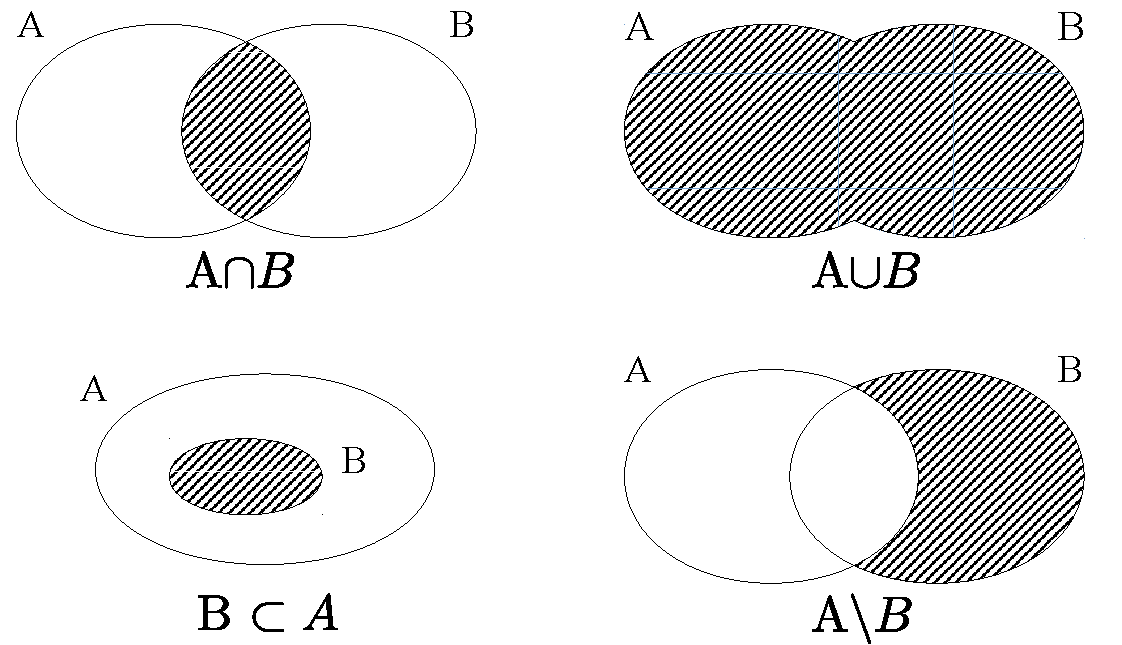
\includegraphics[width=0.7\textwidth, trim={0cm 0cm 0cm
          0cm},clip]{setRelations}
          \caption[]{}
          \label{fig: set relations}
        \end{figure}
      \subsection*{Maps}
        \begin{definition}[Maps between sets]
          Let $A$ and $B$ be two sets. A map $f$ is a many-to-one or
          one-to-one relation between elements in set $A$ and elements in set
          $B$. I.e, $\forall a \in A$, we have a corresponding element $f(a)
          \in B$. We denote a map in one of these two ways:
          \[A \xrightarrow{f} B \quad \quad f: A \rightarrow B\]
        \end{definition}
        \begin{definition}[Images and pre-images]
          Suppose we have $f: A\rightarrow B$. We say that $f(A)$ is the
          image of $A$ under $f$.\\
          We can also define a concept known as the pre-image of a map $f$,
          which we denote as $f^{-1}$. I.e, $\forall b \in B$, we have:
          $f^{-1}(b) = \{a \in A \,|f(a) = b\}$. Note that $f^{-1}$ is not necessarily a map, because $f^{-1}$ can be one-to-many.
        \end{definition}
        \begin{definition}(Injective, Surjective and Bijective)
          \begin{itemize}
            \item{A map $f: A \rightarrow B$ is one-to-one, or injective, if
            $\forall a,b \in A$, $f(a) = f(b) \Leftrightarrow a=b$.}
            \item{A map $f: A \rightarrow B$ is onto, or surjective, if
            $\forall b \in B$, $\exists a \in A$ such that $f(a) = b$. In other words, $f(A) = B$.}
            \item{A map $f: A \rightarrow B$ is bijective if and only if it is both surjective and injective.}
          \end{itemize}
        \end{definition}
        \subsubsection*{Inverse maps and composition of maps}
          Notice that if $f$ is bijective, then $\forall b \in B$, $f^{-1}(b)
          \equiv a \in A$ is a unique element such that $f(a) = b$. In other
          words, if $f$ is a bijective map from $A \rightarrow B$, then
          $f^{-1}$ is a map from $B \rightarrow A$ such that $f \circ f^{-1}$
          is the identity map from $B \rightarrow B$ and $f^{-1} \circ f$ is
          the identity map from $A \rightarrow A$. We call $f^{-1}$ the inverse
          map of $f$.

          Here we have also introduced the composition of two maps, denoted
          by $\circ$. I.e, if \[A \xrightarrow{f} B, B \xrightarrow{g} C\]
          then $g \circ f$ is a map from $A \rightarrow C$.
        \subsubsection*{Useful rules for maps}
          For maps in general, there are some useful rules which are listed below:
          \begin{enumerate}
            \item{Let $f: X\rightarrow Y$ be a map between two sets $X$ and
            $Y$. Then for any subsets $A,B$ of $X$, we can show that:
            \begin{itemize}
              \item{$f(A \cup B) = f(A) \cup f(B)$}
              \item{$f(A \cap B) \subset f(A) \cap f(B)$}
              \item{$f(A \backslash B) \supset f(A) \backslash f(B)$}
            \end{itemize}}
            \item{Let $f: X\rightarrow Y$ be a map between two sets $X$ and
            $Y$. Then for any subsets $A,B$ of $Y$, we can show that:
            \begin{itemize}
              \item{$f^{-1}(A \cup B) = f^{-1}(A) \cup f^{-1}(B)$}
              \item{$f^{-1}(A \cap B) = f^{-1}(A) \cap f^{-1}(B)$}
              \item{$f^{-1}(A \backslash B) = f^{-1}(A) \backslash f^{-1}(B)$}
            \end{itemize}}
          \end{enumerate}
          \begin{proof}
            \textcolor{red}{Coming soon! For now, see Kuldip's tutorial 1.
            This question is quite a standard math question in introductory
            math books...}
          \end{proof}
      \subsection*{Equivalence classes}
      Given a set $A$, we can define an equivalence relation $~$ between
      elements of the set like this: $\forall x,y \in A$, we write $x~y$ if
      $~$ satisfies the following three properties:
      \begin{enumerate}
        \item{Reflexive: $x\sim x$}
        \item{Symmetric: if $x\sim y$ then $y\sim x$}
        \item{Transitive: if $x\sim y$ and $y\sim z$ then $x\sim z$}
      \end{enumerate}
      \begin{theorem}[Fundamental theorem of equivalence relations]
        Let $\sim$ be an equivalence relation on the set $A$. If for every $x
        \in A$ we form the subsets \[B_x = \{y\in A \,|y\sim x\}\] then the
        family of subsets $B_x$ is a partition of $A$. The set $B_x$ is
        called an equivalence class with representative $x$. By partition, we
        mean that:
        \begin{enumerate}
          \item{$A = \bigcup\limits_{x\in A} B_x$}
          \item{If $B_x \cap B_y \neq \phi$ then $B_x = B_y$}
        \end{enumerate}
      \end{theorem}
      \begin{remark}
        By the way, we call the set of all equivalence classes,
        $\{B_x\}_{x\in A}$, denoted by $A\backslash \sim$, the quotient set.
      \end{remark}
      \begin{proof}
        \textcolor{red}{Will fill in soon. For now, just refer to any
        introductory math textbook... (Proof by reference)}
      \end{proof}
    \section{Basics of point-set Topology}
      \begin{definition}[Topology]
        \label{defn: defn of topology}
        A topological structure, or more briefly a topology, on a set $X$ is
        a structure given by a set $\mathcal{D}$ of subsets of $X$ having the
        following properties (called axioms of topological structures):
        \begin{enumerate}
          \item{Every union of sets of $\mathcal{D}$ is a set of
          $\mathcal{D}$}
          \item{Every finite intersection of sets of $\mathcal{D}$ is a set
          of $\mathcal{D}$ \label{item: topology defn axiom 2}}
        \end{enumerate}
      \end{definition}
      \begin{remark} A few remarks are in order:
        \begin{itemize}
          \item{When the cardinality of $X$ is countably/uncountably
          infinite, there might be some difficuly with axiom \ref{item:
          topology defn axiom 2}. This is a technical detail, not that
          important.}
          \item{It is easy to prove that $\phi$ and $X$ are always elements of
          $\mathcal{D}$.}
          \item{The power set $\mathcal{P}(X)$ of $X$ is an example of a
          topology on $X$. The trivial topology $\mathcal{D} = \{\phi, X\}$
          is also a topology on $X$. We can prove this by checking that both
          the power set and the trivial topology satisfies
          defintion~\ref{defn: defn of topology}.}
          \item{The set $X$ together with $\mathcal{D}$ is known as a
          topological space. The elements of $\mathcal{D}$ are known as the
          open sets of this topological space.}
        \end{itemize}
      \end{remark}
    \begin{definition}[Closed sets]
      Given a topological space $(X, \mathcal{D})$, closed sets are the
      complements of open sets.
    \end{definition}
    The above definition of closed sets is if we use definition~\ref{defn:
    defn of topology} as the definition of a topology. If we use
    definition~\ref{defn: alternate defn of topology} instead, then we will
    start with closed sets. Then, open sets would be defined as the
    complements of closed sets.
    \begin{definition}[Alternate definition of a topology]
      \label{defn: alternate defn of topology}
      An alternate definition of a topology can also be given in terms of
      closed sets: Consider the set $\mathcal{D}^\prime$ of subsets of $X$ with
      the following properties:
      \begin{enumerate}
        \item{Every finite union of sets in $\mathcal{D}^\prime$ is a set in
        $\mathcal{D}^\prime$}
        \item{Every intersection of sets in $\mathcal{D}^\prime$ is a set in
        $\mathcal{D}^\prime$}
      \end{enumerate}
      Note that here, $\phi$ and $X$ are also elements of
      $\mathcal{D}^\prime$. Elements of $ \mathcal{D}^\prime$ are known as
      closed sets, and then open sets can be defined as the complement of
      closed sets.
    \end{definition}
    \begin{definition}[Interior points, Exterior points, Boundary points]
      Consider a subset $A$ of a topological space $X$. We can characterise
      $x \in X$ as being either an interior point, exterior point or boundary
      point
      \textcolor{red}{Coming soon!}
    \end{definition}
    \subsection{Metric topology}
      \textcolor{red}{Coming soon!}
    